\documentclass{beamer}
\usepackage[utf8]{inputenc}
\usepackage{tabularx}
\usetheme{Frankfurt}
\newcommand\TestAppExists[3]{#2}
\usepackage{minted}
\usepackage{listings}
\usepackage{media9}

\usepackage{pgf}
\usepackage{tikz}
\usetikzlibrary{arrows,automata}
\usepackage{tikz-cd}
\usetikzlibrary{positioning}

   
\usepackage{mathpartir}
\usepackage{multicol}
\usepackage{graphicx}


\lstset{ %
	basicstyle=\small\ttfamily,
	breakatwhitespace=true,
	breaklines=false,
	commentstyle=\color{green!40!black},
	extendedchars=true, 
	keepspaces=true, 
	keywordstyle=\color{blue},
	showspaces=false,               
	showstringspaces=false,         
	showtabs=false,
	tabsize=2
}
  
  \setbeamerfont{institute}{size=\fontsize{7pt}{8pt}}
  
  \title{Copilot : Traceability and Verification of a Low Level Automatically Generated C Source Code}
  \author{Georges-Axel Jaloyan}
  \institute{\'Ecole Normale Sup\'erieure, NASA Langley Research center, National Institute of Aerospace}
  \date{August 12, 2015}
  
\begin{document}
\begin{frame}
  		
  		\titlepage
  		\begin{center}
  			\includegraphics[height=2cm]{images/ENS-logo.jpg} \includegraphics[height=2cm]{images/NASA.png}
  			\includegraphics[height=2cm]{images/NIA-logo.jpg}
  		\end{center}
\end{frame}
  	
  	
  	\section{Preliminaries}
  	\subsection{Copilot language}
\begin{frame}
  		\tableofcontents[currentsubsection,sectionstyle=show/shaded,subsectionstyle=show/shaded/hide]
\end{frame}
  	
\begin{frame}
  		\frametitle{Copilot language}
  		Copilot is an \emph{EDSL} (embedded domain specific language), embedded in \emph{Haskell} and used for writing \emph{runtime monitors} for hard real-time, distributed, reactive systems written in C. 
  		\\~\\
  		\text{A Copilot program, can either be : } 
  		\begin{itemize}
  			\item compiled to C using two back-ends : SBV, ATOM
  			\item interpreted
  			\item analyzed using static analysis tools (CBMC, Kind)
  		\end{itemize} 
\end{frame}
  	
\begin{frame}[fragile]
  		\frametitle{Copilot syntax}
  		A program is a list of streams that can be either external  or internal which are defined by mutually recursive stream equations.
  		\\~\\
  		Each stream has a type which can be \texttt{Bool}, \texttt{Int8}, \texttt{Int16}, \texttt{Int32}, \texttt{Int64}, \texttt{Word8}, \texttt{Word16}, \texttt{Word32}, \texttt{Word64}, \texttt{Float}, \texttt{Double}.
  		
\begin{minted}{haskell}
x :: Stream Word16
x = 0
-- x = {0, 0, 0, ...}
y :: Stream Bool
y = x `mod` 2 == 0
-- y = {T, T, ...}
nats :: Stream Word64
nats = [0] ++ (1 + nats)
-- nats = {0,1,2, ..., 2^64-1, 0, 1, ..}  
\end{minted}
\end{frame}
  	
\begin{frame}[fragile]
	\frametitle{Operators}
  		Each operator and constant has been lifted to Streams (working pointwise). \\~\\
  		Two temporal operations working on Streams : 
  		\begin{itemize}
  			\item ++ : which prepends a finite list to a Stream

\begin{minted}{haskell}
(++) :: [a] -> Stream a -> Stream a
\end{minted}
  			\item drop : which drops a finite number of elements at the beginning of a Stream
\begin{minted}{haskell}
drop :: Int -> Stream a -> Stream a  
\end{minted}
  		\end{itemize}
  		
Casts and unsafe casts are also provided :
\begin{minted}{haskell}
cast :: (Typed a, Typed b) => Stream a -> Stream b
unsafeCast :: (Typed a, Typed b) => Stream a -> Stream b
\end{minted}
\end{frame}
  	
\begin{frame}[fragile]
  		\frametitle{Examples}
	Fibonacci sequence :
\begin{minted}{haskell}
fib :: Stream Word64
fib = [1,1] ++ (fib + drop 1 fib) 
-- fib = {1,1,2,3,5,8,13,...,
--       12200160415121876738,
--   /!\ 1293530146158671551,...}
\end{minted}

\end{frame}

\begin{frame}[fragile]
	\frametitle{Interaction}
	Sensors :
	\begin{itemize}
		\item<1|only@1> Sample external variables. 
\begin{minted}{haskell}
extern :: Typed a => String -> Maybe [a] -> Stream a
\end{minted}
Example : 
\begin{lstlisting}[language=C]
unsigned long long int x;
\end{lstlisting}
\begin{minted}{haskell}
x :: Stream Word64
x = extern "x" (Just [0,0..])

x2 = externW64 "x" Nothing
\end{minted}

		\item<2-4> Sample external variables. 
		\item<2|only@2> Sample external arrays. 
\begin{minted}{haskell}
externArray :: (Typed a, Typed b, Integral a) => 
String -> Stream a -> Int -> Maybe [[a]] -> Stream b
\end{minted}
Example : 
\begin{lstlisting}[language=C]
unsigned long long int tab[1000];
\end{lstlisting}
\begin{minted}{haskell}
-- nat = [0] ++ (nats + 1)
x :: Stream Word64
x = externArray "tab" nats 1000 Nothing

x2 = externArrayW64 "tab" nats 1000 Nothing
\end{minted}
	
		\item<3-4> Sample external arrays. 
		\item<3|only@3> Sample external functions. 

\begin{minted}{haskell}
externFun :: Typed a => 
String -> [FunArg] -> Maybe [a] -> Stream a
\end{minted}
Example :
\begin{lstlisting}[language=C]
double sin(double a); //from math.h
\end{lstlisting}
\begin{minted}{haskell}
x :: Stream Double
x = externDouble "x" Nothing

sinx = externFun "sin" [arg x] Nothing
\end{minted}
		
		\item<4> Sample external functions. 
	\end{itemize}
\end{frame}
  	
\begin{frame}[fragile]
  		\frametitle{Interaction}
  		
	Actuators :
  	\begin{itemize}
		\item Triggers : 
\begin{minted}{haskell}
trigger :: 
  String -> Stream Bool -> [TriggerArg] -> Spec
\end{minted}
		\item Observers :
\begin{minted}{haskell}
observer :: Typed a => String -> Stream a -> Spec
\end{minted}
	\end{itemize}
\end{frame}
  	
  	\subsection{ACSL}
  	\begin{frame}
  		\tableofcontents[currentsubsection,sectionstyle=show/shaded,subsectionstyle=show/shaded/hide]
  	\end{frame}
  	
\begin{frame}[fragile]
	\frametitle{ACSL syntax}
	ACSL is a specification language for C programs. Those contracts are written according to the following example :
\begin{lstlisting}[language=C]
/*@ requires true
assigns \nothing
ensures \result >= x && \result >= y;
ensures \result == x || \result == y;
*/
int max (int x, int y) { return (x > y) ? x : y; }
\end{lstlisting}
	
\end{frame}
  	
\begin{frame}[fragile]
	\frametitle{Floyd-Hoare logic}
	A Floyd-Hoare triple is : \\
	$\lbrace P \rbrace~ prog ~\lbrace Q \rbrace$ \\
	\begin{itemize}
		\item $prog$ is a program fragment
		\item $P$ and $Q$ are logical assertions over program variables 
		\item $P$ is the precondition
		\item $Q$ the postcondition
	\end{itemize}
	
	$\lbrace P \rbrace~ prog ~\lbrace Q \rbrace$ holds iff
	\begin{itemize}
		\item $P$ holds before the execution of $prog$
		\item $Q$ holds after the execution of $prog$\footnote{Unless $prog$ does not terminate or encounters an error.}
	\end{itemize}

\end{frame}
	
\begin{frame}[fragile]
	\frametitle{Floyd-Hoare logic}
	Here is an example of a proof tree of a program\footnote{A. Min\'e, \textit{"Semantics and application to program verification : Axiomatic semantics"}, 2015.}:
	\[
	\inferrule* []
	{\inferrule* [] {\inferrule* [] {\inferrule* [] { }
				{\lbrace true \rbrace~ I \leftarrow I - 1 \ ~\lbrace true\rbrace}}
			{\lbrace I \ne 0 \rbrace~ I \leftarrow I - 1 \ ~\lbrace true \rbrace}}
		{\lbrace true \rbrace~  \texttt{while} ~ I \ne 0 ~ \texttt{do} ~ I \leftarrow I - 1 \ ~\lbrace true \wedge \neg (I \ne 0) \rbrace}
	}
	{\lbrace true \rbrace~  \texttt{while} ~ I \ne 0 ~ \texttt{do} ~ I \leftarrow I - 1 \ ~\lbrace I = 0 \rbrace}
	\]
\end{frame}

\begin{frame}[fragile]
	\frametitle{Floyd-Hoare logic}
	The Floyd-Hoare logic does not take into account program termination:
	\[
	\inferrule* []
	{\inferrule* [] {\inferrule* [] {\inferrule* [] { }
				{\lbrace true \rbrace~ I \leftarrow I \ ~\lbrace true\rbrace}}
			{\lbrace I \ne 0 \rbrace~ I \leftarrow I \ ~\lbrace true \rbrace}}
		{\lbrace true \rbrace~  \texttt{while} ~ I \ne 0 ~ \texttt{do} ~ I \leftarrow I \ ~\lbrace true \wedge \neg (I \ne 0) \rbrace}
	}
	{\lbrace true \rbrace~  \texttt{while} ~ I \ne 0 ~ \texttt{do} ~ I \leftarrow I ~\lbrace I = 0 \rbrace}
	\]
\end{frame}

\begin{frame}[fragile]
	\frametitle{Floyd-Hoare logic}
	Or even safety against runtime errors (we speak about partial correctness):
	\[
	\inferrule* []
	{\inferrule* [] {\inferrule* [] {\inferrule* [] { }
				{\lbrace true \rbrace~ \textbf{fail} \ ~\lbrace true\rbrace}}
			{\lbrace I \ne 0 \rbrace~ \textbf{fail} \ ~\lbrace true \rbrace}}
		{\lbrace true \rbrace~  \texttt{while} ~ I \ne 0 ~ \texttt{do} ~ \textbf{fail} \ ~\lbrace true \wedge \neg (I \ne 0) \rbrace}
	}
	{\lbrace true \rbrace~  \texttt{while} ~ I \ne 0 ~ \texttt{do} ~ \textbf{fail} ~\lbrace I = 0 \rbrace}
	\]
	
	More generally, any property is true after fail :
	\[
	\inferrule* [] { }
	{\lbrace P \rbrace~ \textbf{fail} ~\lbrace Q \rbrace}
	\]
\end{frame}

\begin{frame}[fragile]
	\frametitle{Floyd-Hoare logic}
	It is nevertheless possible to prove total correctness by the following proof tree (ranking functions have to be provided):
	\[
	\inferrule* []
	{\lbrace P \rbrace~  prog ~\lbrace Q \rbrace \\ \lbrack P \rbrack~  prog ~\lbrack true \rbrack
	}
	{\lbrack P \rbrack~  prog~ \lbrack Q \rbrack}
	\]
\end{frame}

\begin{frame}[fragile]
	\frametitle{Dijkstra's Weakest Liberal Precondition}
	We define the weakest liberal precondition : $wlp(prog,Q)$  which is defined as the most general condition such that $\lbrace wlp(prog,Q) \rbrace~  prog~ \lbrace Q \rbrace$ holds.\\~\\
	We can automate the computation of the precondition by induction on the syntax. 
	\begin{itemize}
		\item $wlp(skip, P) = P$
		\item $wlp(fail, P) = true$
		\item $wlp(s;t, P) = wlp(s, wlp(t, P))$
		\item $wlp(X \leftarrow e, P) = P[e/X]$
		\item $wlp(\texttt{if}~e~\texttt{then}~s~\texttt{else}~t,P) = (e \Rightarrow wlp(s, P)) \wedge (\neg e \Rightarrow wlp(t, P))$ 
	\end{itemize}
	
\end{frame}

  	\subsection{Copilot toolchain}
  	\begin{frame}
  		\tableofcontents[currentsubsection,sectionstyle=show/shaded,subsectionstyle=show/shaded/hide]
  	\end{frame}

\begin{frame}[fragile]
\begin{figure}[ht!]
	\centering
	\footnotesize
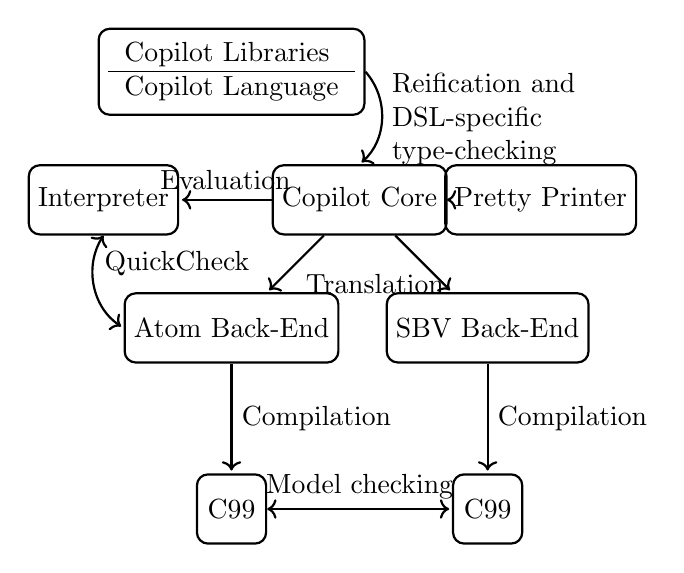
\begin{tikzpicture}[->, node distance=2.3cm, auto, shorten >=1pt, bend angle=45,thick]
\tikzstyle{every state}=[rectangle, rounded corners]
	
	
\node[state] (Int) {Interpreter};
\node[state] (Lang) [above right of=Int]
{
	\begin{tabular}[b]{l}
	Copilot Libraries\\ \hline Copilot Language
	\end{tabular}};
\node[state] (Core) [below right of=Lang] {Copilot Core};
\node[state] (PP) [right of=Core] {Pretty Printer};
		
		
\node[state] (Atom) [below left of=Core] {Atom Back-End};
\node[state] (SBV) [below right of=Core] {SBV Back-End};
\node[state] (C99A) [below of=Atom] {C99};
\node[state] (C99S) [below of=SBV] {C99};
		
		
\tikzstyle{every node}=[]
		
		
\path %% (Libs) edge node {0,1,L} (Lang);
%% edge node {1,1,R} (C)
(Lang) edge [bend left, anchor=west, text width=2.5cm] node {Reification and DSL-specific type-checking} (Core)
%% edge node {0,1,L} (C)
(Core) edge node {Translation} (Atom)
edge node {} (SBV)
edge node {} (PP)
edge node [swap] {Evaluation} (Int)
(Int) edge [<->, bend right] node {QuickCheck} (Atom)
(Atom) edge node {Compilation} (C99A)
(SBV) edge node {Compilation} (C99S)
(C99A) edge [<->] node {Model checking} (C99S);
%% edge [bend left] node {Translation} (SBV)
%% (Atom) edge [loop below] node {1,1,R} (D)
%% edge node {0,1,R} (Libs)
%% (SBV) edge [bend left] node {1,0,R} ();
\end{tikzpicture}
\caption{The Copilot toolchain\footnote{L. Pike, N. Wegmann, S. Niller, and A. Goodloe, \textit{Experience report: A do-it-yourself high-assurance compiler}, 2012.}}
	\end{figure}
\end{frame}
  	
  	  	\section{Working on the backend}
  	  	\subsection{Hand-written ACSL}
  	  	\begin{frame}
  	  		\tableofcontents[currentsubsection,sectionstyle=show/shaded,subsectionstyle=show/shaded/hide]
  	  	\end{frame}
  	
  	
\begin{frame}[fragile]
\frametitle{Hand written ACSL}

\begin{minted}{haskell}
import Copilot.Language.Reify
import Copilot.Language
import qualified Copilot.Compile.SBV as S
  	
logic :: Stream Bool
logic = [True, False] ++ logic && drop 1 logic
  	
spec :: Spec
spec = do
observer "obs1" logic
  	
main = do
interpret 10 spec
reify spec >>= S.compile S.defaultParams --SBV Backend
  	
\end{minted}
  	
\end{frame}
\begin{frame}[fragile]
	\scriptsize 
\begin{lstlisting}[language=C, keywordstyle=\color{blue}]
/*@
requires ptr_2 < 0x0078;
requires \valid(queue_2 + (0..0x02U-1));
assigns \nothing;
ensures \result == ( queue_2[ptr_2 % 0x02U] 
                && queue_2[(ptr_2 + 0x01U) % 0x02U]);
*/
SBool update_state_2(const SBool *queue_2
                    , const SWord16 ptr_2)
{
  const SWord16 s2 = ptr_2;
  const SWord16 s4 = (0x02U == 0)?s2:(s2%0x02U);
  const SBool   s5 = queue_2[s4];
  const SWord16 s7 = s2 + 0x0001U;
  const SWord16 s8 = (0x02U == 0)?s7:(s7%0x02U);
  const SBool   s9 = queue_2[s8];
  const SBool   s10 = s5 && s9;
  	
  return s10;
}
\end{lstlisting}


\end{frame}
\begin{frame}[fragile]
  	\texttt{frama-c -wp -wp-out . -wp-prover PROVER}
  	
\begin{lstlisting}[]
[wp] Proved goals:   19 / 19
Qed:            18  (4ms-4ms)
cvc4:            1  (150ms-150ms)

[wp] Proved goals:   19 / 19
Qed:            18  (4ms-4ms)
cvc3:            1  (90ms-90ms)
	
[wp] Proved goals:   19 / 19
Qed:            18  (4ms-8ms)
Alt-Ergo:        1  (3.5s-3.5s) (248)

[wp] Proved goals:   19 / 19
Qed:            18  (4ms-4ms)
z3:              1  (20ms-20ms)
\end{lstlisting}
  	
\end{frame}

\begin{frame}[fragile]
	\scriptsize 
	Bitwise version : 
\begin{lstlisting}[language=C]
/*@
requires ptr_2 < 0x0078;
requires \valid(queue_2 + (0..0x02U-1));
assigns \nothing;
ensures \result == ( queue_2[ptr_2 % 0x02U] 
& queue_2[(ptr_2 + 0x01U) % 0x02U]);
*/
SBool update_state_2(const SBool *queue_2
, const SWord16 ptr_2)
{
const SWord16 s2 = ptr_2;
const SWord16 s4 = (0x02U == 0)?s2:(s2%0x02U);
const SBool   s5 = queue_2[s4];
const SWord16 s7 = s2 + 0x0001U;
const SWord16 s8 = (0x02U == 0)?s7:(s7%0x02U);
const SBool   s9 = queue_2[s8];
const SBool   s10 = s5 & s9;

return s10;
}
\end{lstlisting}
	
	
\end{frame}
\begin{frame}[fragile]
	\texttt{frama-c -wp -wp-out . -wp-prover PROVER}
	
\begin{lstlisting}[]
[wp] Proved goals:   15 / 16
Qed:            15  (4ms-4ms)
cvc4:            0  (interrupted: 1)

[wp] Proved goals:   15 / 16
Qed:            15  (4ms-4ms)
cvc3:            0  (unknown: 1)

[wp] Proved goals:   15 / 16
Qed:            15  (4ms-4ms)
Alt-Ergo:        0  (interrupted: 1)

[wp] Proved goals:   15 / 16
Qed:            15  (4ms-4ms)
z3:              0  (interrupted: 1)    
----> Timeout after 30 seconds

\end{lstlisting}
	
\end{frame}

\begin{frame}[fragile]
	\scriptsize 
	Unsafe version : 
\begin{lstlisting}[language=C]
/*@
requires \valid(queue_2 + (0..0x02U-1));
assigns \nothing;
ensures \result == ( queue_2[ptr_2 % 0x02U] 
&& queue_2[(ptr_2 + 0x01U) % 0x02U]);
*/
SBool update_state_2(const SBool *queue_2
, const SWord16 ptr_2)
{
const SWord16 s2 = ptr_2;
const SWord16 s4 = (0x02U == 0)?s2:(s2%0x02U);
const SBool   s5 = queue_2[s4];
const SWord16 s7 = s2 + 0x0001U;
const SWord16 s8 = (0x02U == 0)?s7:(s7%0x02U);
const SBool   s9 = queue_2[s8];
const SBool   s10 = s5 && s9;

return s10;
}
\end{lstlisting}

	
	
\end{frame}
\begin{frame}[fragile]
	\texttt{frama-c -wp -wp-out . -wp-prover PROVER}
	
\begin{lstlisting}[]
[wp] Proved goals:   18 / 19
Qed:            18  (4ms-4ms)
cvc4:            0  (interrupted: 1)

[wp] Proved goals:   18 / 19
Qed:            18  (4ms-4ms)
Alt-Ergo:        0  (interrupted: 1)

[wp] Proved goals:   18 / 19
Qed:            18  (4ms-4ms)
z3:              0  (unknown: 1)   
----> NO TIMEOUT : unsafe
\end{lstlisting}
	
\end{frame}

\subsection{ACSL generation}
\begin{frame}
	\tableofcontents[currentsubsection,sectionstyle=show/shaded,subsectionstyle=show/shaded/hide]
\end{frame}


\begin{frame}[fragile]
\frametitle{ACSL generation}
The easiest way to do it is by induction on the syntax, when compiling the expression. Here is how the function ppACSL is constructed :
\begin{itemize}
	\item $\texttt{Const~type~value} \rightarrow show~\texttt{value}$
	\item $\texttt{Drop~type~i~id} \rightarrow queue\_\texttt{id} \lbrack ptr\_\texttt{id} + \texttt{i} ~ mod ~ (length~\texttt{id}) \rbrack$
	\item $\texttt{ExternVar~t~name~b} \rightarrow ext\_\texttt{name}$
	\item $\texttt{Var type name} \rightarrow \texttt{name}$
	\item $\texttt{Op2 op e1 e2} \rightarrow (ppACSL~\texttt{e1})~show~\texttt{op}~(ppACSL~\texttt{e2})$
	\item $\texttt{Label~t~s~e} \rightarrow ppACSL~\texttt{e}$
\end{itemize}
\end{frame}

\begin{frame}[fragile]
\frametitle{ACSL generation}
Nevertheless, some hacks :

\begin{itemize}
	\item Let bindings have been deprecated.
	\item Abs are converted to $\backslash a \rightarrow sign~a \times a$
	\item Sign to $\backslash x \rightarrow ((x > 0)~?~1 : ((x < 0) ? -1 : 0))$
	\item Mux where branches have type Bool to $Mux~e1~e2~e3 = ( e2 \wedge e1) \vee (e3 \wedge \neg e1)$
	\item No bitwise operator are supported.
\end{itemize}
\end{frame}

\begin{frame}[fragile]
	\frametitle{ACSL generation}
	Still some problems with frama-c :
	
	\begin{itemize}
		\item No global invariant : we have to split the dereferencing of the pointer into a black box that only do this.
		\item No math functions (such as sin, cos, exp, log, ...) : we have to do the same.
	\end{itemize}
\end{frame}

\begin{frame}[fragile]
	\frametitle{WP vs VA}
	How effective value analysis is ?
	\begin{itemize}
		\item Global invariants supported
		\item No lemma supported
		\item Safe ... for only one iteration of the main loop
		\item Does not really go well with external variables
		\item Requires access to all C source files of the project to say anything about one contract.
	\end{itemize}
	(Very bad) solution : unroll the infinite loop ! \\
	\texttt{frama-c -val -main testing -slevel 10000000 *.h *.c}
	(Better) solution : forget about value analysis for the monitor.
\end{frame}

\begin{frame}[fragile]
	\frametitle{Other changes}
	\begin{itemize}
		\item Added m4 preprocessing
		\item Added CompCert for compiling the C source file generated
		\item Deprecated ATOM
		\item Added a dot graph generation for each source file.
	\end{itemize}
\end{frame}

\begin{frame}[fragile]
	\frametitle{Dot File: "ext\_ident\_bool\_1789\_arg0.c"}
	\footnotesize 
\begin{lstlisting}[language=C]
/*@
assigns \nothing;
ensures \result == 
      ((((((0.0) <= (ext_ident_double_1778))) 
      && (((ext_ident_double_1788) <= (0.0))))));
*/
SBool ext_ident_bool_1789_arg0
(const SDouble ext_ident_double_1778,
const SDouble ext_ident_double_1788)
{
  const SDouble s0 = ext_ident_double_1778;
  const SDouble s14 = ext_ident_double_1788;
  const SBool   s25 = 0.0 <= s0;
  const SBool   s26 = s14 <= 0.0;
  const SBool   s27 = s25 && s26;
  const SBool   s28 = s27 /* vertical_RA */;
  return s28;
}
\end{lstlisting}
\end{frame}

\begin{frame}[fragile]
	\frametitle{Dot File: "ext\_ident\_bool\_1789\_arg0.c"}
	An example of a dot graph associated to a C source file.\\
	\begin{figure}
		\includegraphics[width=100mm]{images/graph.ps}
	\end{figure}
	
\end{frame}

\begin{frame}[fragile]
	\frametitle{Magic labels}
	The possibility to add labels that would be printed in the C source file was also added in SBV and in Copilot. \\~\\
	The prover was not able to prove long expressions (some were 500000 characters long).\\~\\
	So we need to add a special instruction that has one only role : split the AST into smaller ones that can be easily provable. This instruction has to be totally useless regarding to the semantics of the language. Labels do not change the semantics of the program. So why not using them ? \\~\\
	The idea is to call the function identity when we encounter a magic label. This is equivalent to the transformation : $ e \rightarrow_{\beta} (\lambda x . x) e $. 

\end{frame}

\begin{frame}[fragile]
	\frametitle{Magic labels: example}
\begin{minted}{haskell}
import qualified Copilot.Compile.SBV as S

alt :: Stream Bool
alt = (label "?splitting" $ not $ 
      externB "externvar" Nothing)

spec :: Spec
spec = do
trigger "trigger" (alt) []

main = do
reify spec >>= S.proofACSL S.defaultParams
\end{minted}


\end{frame}

\begin{frame}[fragile]
	\frametitle{Magic labels: example}
	~\\
	\begin{figure}
		\includegraphics[width=33mm]{images/label/main.ps}
		\centering
		\includegraphics[width=33mm]{images/label/splitted.ps}
		\includegraphics[width=33mm]{images/label/splitted2.ps}
	\end{figure}
	
\end{frame}

\begin{frame}[fragile]
	\begin{figure}[ht!]
		\centering
		\footnotesize
		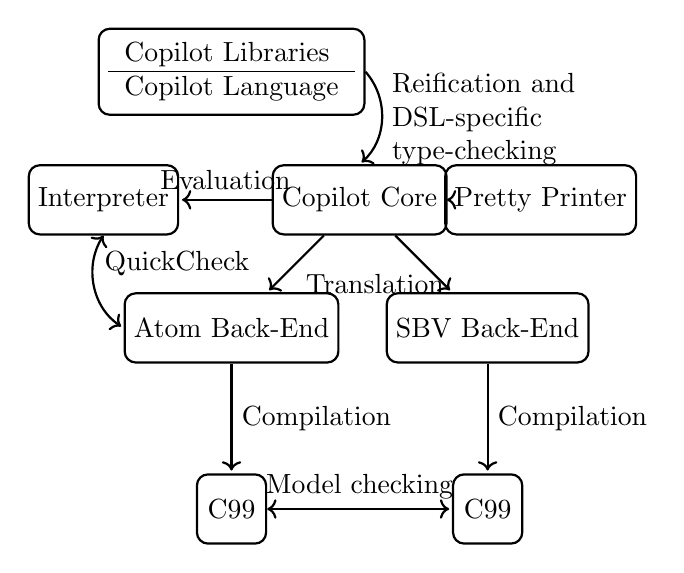
\begin{tikzpicture}[->, node distance=2.3cm, auto, shorten >=1pt, bend angle=45,thick]
		\tikzstyle{every state}=[rectangle, rounded corners]
		
		
		\node[state] (Int) {Interpreter};
		\node[state] (Lang) [above right of=Int]
		{
			\begin{tabular}[b]{l}
			Copilot Libraries\\ \hline Copilot Language
			\end{tabular}};
		\node[state] (Core) [below right of=Lang] {Copilot Core};
		\node[state] (PP) [right of=Core] {Pretty Printer};
		
		
		\node[state] (Atom) [below left of=Core] {Atom Back-End};
		\node[state] (SBV) [below right of=Core] {SBV Back-End};
		\node[state] (C99A) [below of=Atom] {C99};
		\node[state] (C99S) [below of=SBV] {C99};
		
		
		\tikzstyle{every node}=[]
		
		
		\path %% (Libs) edge node {0,1,L} (Lang);
		%% edge node {1,1,R} (C)
		(Lang) edge [bend left, anchor=west, text width=2.5cm] node {Reification and DSL-specific type-checking} (Core)
		%% edge node {0,1,L} (C)
		(Core) edge node {Translation} (Atom)
		edge node {} (SBV)
		edge node {} (PP)
		edge node [swap] {Evaluation} (Int)
		(Int) edge [<->, bend right] node {QuickCheck} (Atom)
		(Atom) edge node {Compilation} (C99A)
		(SBV) edge node {Compilation} (C99S)
		(C99A) edge [<->] node {Model checking} (C99S);
		%% edge [bend left] node {Translation} (SBV)
		%% (Atom) edge [loop below] node {1,1,R} (D)
		%% edge node {0,1,R} (Libs)
		%% (SBV) edge [bend left] node {1,0,R} ();
		\end{tikzpicture}
	\end{figure}
\end{frame}
  	
  	
\begin{frame}[fragile]
	\begin{figure}[ht!]
		\centering
		\tiny
		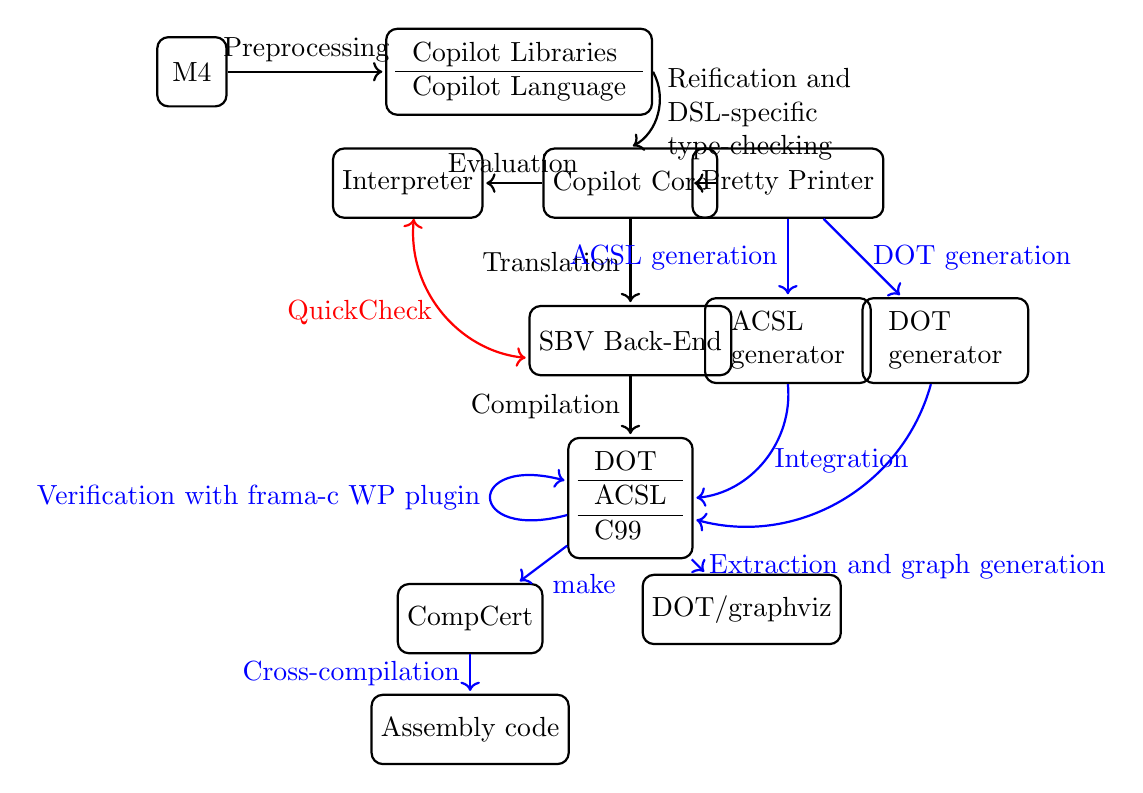
\begin{tikzpicture}[->, node distance=2cm, auto, shorten >=1pt, bend angle=45,
		thick]
		\tikzstyle{every state}=[rectangle, rounded corners]
		
		
		\node[state] (Int) {Interpreter};
		\node[state] (Lang) [above right of=Int]
		{
			\begin{tabular}[b]{l}
			Copilot Libraries\\ \hline Copilot Language
			\end{tabular}};
		
		\node[state] (M4) [left=2cm of Lang] {M4};
		\node[state] (Core) [below right of=Lang] {Copilot Core};
		\node[state] (PP) [right of=Core] {Pretty Printer};
		
		
		\node[state] (ACSL) [below of=PP] {\begin{tabular}[b]{l}
			ACSL\\ generator
			\end{tabular}};
		\node[state] (DOTc) [right of=ACSL] {\begin{tabular}[b]{l}
			DOT\\ generator
			\end{tabular}};
		\node[state] (SBV) [below of=Core] {SBV Back-End};
		\node[state] (C99S) [below of=SBV] {\begin{tabular}[b]{l}
			DOT\\ \hline ACSL\\ \hline C99
			\end{tabular}};
		\node[state] (DOT) [below right of=C99S] {DOT/graphviz};
		\node[state] (CCOMP) [below left=0.3cm and 0.3cm of C99S] {CompCert};
		\node[state] (ASM) [below=0.5cm of CCOMP] {Assembly code};
		
		
		\tikzstyle{every node}=[]
		
		
		\path %% (Libs) edge node {0,1,L} (Lang);
		%% edge node {1,1,R} (C)
		(Lang) edge [bend left, anchor=west, text width=2.5cm] node {Reification and DSL-specific type-checking} (Core)
		%% edge node {0,1,L} (C)
		(M4) edge [] node {Preprocessing} (Lang)
		(Core) edge [anchor=east] node {Translation} (SBV)
		edge node {} (PP)
		edge node [swap] {Evaluation} (Int)
		(ACSL) edge [bend left, anchor=west, blue] node {Integration} (C99S)
		(DOTc) edge [bend left, anchor=east, blue] node {} (C99S)
		(Int) edge [<->,red, bend right, anchor=east] node {QuickCheck} (SBV)
		(PP) edge [->,blue, anchor=east] node {ACSL generation} (ACSL)
		(PP) edge [->,blue, anchor=west] node {DOT generation} (DOTc)
		(C99S) edge [->,blue, anchor=north west] node {make} (CCOMP)
		(CCOMP) edge [->,blue, anchor=east] node {Cross-compilation} (ASM)
		(C99S) edge [loop left, ->,blue, anchor=east] node {Verification with frama-c WP plugin} (C99S)
		(C99S) edge [->,blue, anchor=west] node {Extraction and graph generation} (DOT)
		(SBV) edge [->,anchor=east] node {Compilation} (C99S);
		%% edge [bend left] node {Translation} (SBV)
		%% (Atom) edge [loop below] node {1,1,R} (D)
		%% edge node {0,1,R} (Libs)
		%% (SBV) edge [bend left] node {1,0,R} ();
		\end{tikzpicture}
	\end{figure}
\end{frame}


\subsection{Bug finding}
\begin{frame}
	\tableofcontents[currentsubsection,sectionstyle=show/shaded,subsectionstyle=show/shaded/hide]
\end{frame}

\begin{frame}[fragile]
	\frametitle{And it works !}
	Some front-end bugs :
\begin{itemize}
	\item A reduction of $2^x$ to $2 << x$ instead of $1 << x$.
	\item A reduction of $0^0$ to $0$ instead of $1$.
	\item A reduction of $0^x$ to $0$ instead of $mux (x==0) (1) (0)$.
\end{itemize}
	
\end{frame}

\begin{frame}[fragile]
	\frametitle{Backend bug}
	
	A major SBV back-end bug (never detected by model checking). In a 900 characters long contract of a 100 lines of C code file :
	
\begin{lstlisting}[language=C]
/*@
ensure s27 == 
  ((ext_sqrt_0) / (ext_max_time_for_hor_violation));
*/
SBool trigger(...)
{
  const SDouble s11 = ext_max_time_for_hor_violation;
  const SDouble s13 = ext_sqrt_1;
  const SDouble s27 = s13 / s11;
}  
\end{lstlisting}
	
\end{frame}

\begin{frame}[fragile]
	\frametitle{Backend bug}
	
	This similar bug can be generated with the following haskell code :
\begin{minted}{haskell}
x = externFun "f" [arg 0]
y = externFun "f" [arg 1]
s :: Stream Double
s = x + (y + x)
\end{minted}

\begin{lstlisting}[language=C, keywordstyle=\color{blue}]
/*@
ensure \result == 
   ((ext_f_0) + ((ext_f_1) + (ext_f_0)));
*/
SBool trigger(...)
{
  const SDouble s0 = ext_f_0;
  const SDouble s1 = ext_f_1;
  const SDouble s2 = s1 + s1;  // should be s1 + s0;
  const SDouble s3 = s0 + s2;
  return s3;
}  
\end{lstlisting}
\end{frame}

\section{Applications}
\subsection{Self-separation criteria}
\begin{frame}
	\tableofcontents[currentsubsection,sectionstyle=show/shaded,subsectionstyle=show/shaded/hide]
\end{frame}


\begin{frame}[fragile]
	\frametitle{Self-separation criterion}
	We use the criterion defined in \textit{State-Based Implicit Coordination
	and Applications} by Anthony J. Narkawicz and C\'esar A. Mu\~{n}oz.

	The implementation is 262 lines long, generating in prover mode 433 source files, that are verified by frama-c in 2 min and 39 sec on an intel i5-4200U using the following bash command (which uses GNU parallel) : 
\begin{lstlisting}
parallel frama-c -wp -wp-out . -wp-timeout 20 
-wp-prover CVC4 -wp-split {} ::: *.c | tee 
>logfwp >(grep 'Proved\|Unknown\|Timeout\|Failed
\|Qed:\s\|CVC4:\s\|Parsing .*\.c' > logfwpcompact) 
>(grep 'Proved\|Qed:\s\|CVC4:\s\|Unknown\|Timeout
\|Failed\|Parsing .*\.c')
\end{lstlisting}
	
	In compiling mode, the copilot toolchain generates only 19 files, which are compiled in less than a second with CompCert.
\end{frame}


\subsection{TCAS II}
\begin{frame}
	\tableofcontents[currentsubsection,sectionstyle=show/shaded,subsectionstyle=show/shaded/hide]
\end{frame}

\begin{frame}[fragile]
	\frametitle{TCAS II}
	TCAS II (Traffic alert and Collision Avoidance System). Two parts 
	\begin{itemize}
		\item \emph{Traffic Advisory} (TA) which triggers an audible alert if two planes are too close from each other.
		\item \emph{Resolution Advisory} (RA) which sends instructions to the pilot in order to avoid collision and recover a safe separation between the two planes. Only instructions about vertical speeds and positions are sent.
	\end{itemize}
	
	The TA starts emitting alerts if the intruder plane enters in a safe cylinder (called the TA region) of typically 3.3 nautical miles (nm), which corresponds to 40 seconds before collision. 
	
	The RA is triggered if the conflicts occurs in the RA region, which typically corresponds to 2.1 nm (or 25 sec).  
\end{frame}

\begin{frame}[fragile]
\includemedia[activate=pageopen,width=300pt,height=200pt,addresource=images/TCAS.mp4, flashvars={source=images/TCAS.mp4}]{}{VPlayer.swf}
\end{frame}

\begin{frame}[fragile]
	\frametitle{TCAS II}
	We use the TCAS II implementation in PVS and detailed in \textit{A TCAS-II Resolution Advisory Detection Algorithm} by C\'esar A. Mu\~{n}oz, Anthony J. Narkawicz and James Chamberlain. \\~\\	
	We implemented the alert trigger, and the corrective trigger.
	Both are 447 lines long. \\~\\
	Alert only version :
\begin{itemize}
\item Proof mode : 150 files verified in 13 min and 8 sec
\item Compile mode : 4 files compiled in 2 sec
\end{itemize}
Corrective trigger version :
\begin{itemize}
\item Proof mode : 1790 files verified in 4h38.
\item Compile mode : 5 files compiled in 2 sec
\end{itemize}
	
\end{frame}

\subsection{Well-Clear}
\begin{frame}
	\tableofcontents[currentsubsection,sectionstyle=show/shaded,subsectionstyle=show/shaded/hide]
\end{frame}


\begin{frame}[fragile]
	\frametitle{Well-Clear}
	
	Last implementation : Well-Clear criterion defined in \textit{A Family of Well-Clear Boundary Models for the Integration of UAS in the NAS} by C\'esar A. Mu\~{n}oz, Anthony J. Narkawicz and James Chamberlain, Mar\'ia Consiglio and Jason Upchurch.
	
	\begin{figure}
		\includegraphics[height=16mm]{images/WCV/tau.pdf}\\
		\includegraphics[height=16mm]{images/WCV/tcpa.pdf}\\
		\includegraphics[height=16mm]{images/WCV/taumod.pdf}\\
	\end{figure}
	

\end{frame}

\begin{frame}[fragile]
	\frametitle{Well-Clear}

	
	\begin{figure}
		\includegraphics[height=15mm]{images/WCV/tep.pdf}\\
	\end{figure}
		where
	\begin{figure}
		\includegraphics[height=15mm]{images/WCV/theta.pdf}\\
	\end{figure}
	
\end{frame}

\begin{frame}[fragile]
	\frametitle{Well-Clear}
	
	
	\begin{figure}
		\includegraphics[height=30mm]{images/WCV/wcv.pdf}\\
	\end{figure}
	where
	\begin{figure}
		\centering
		\includegraphics[height=18mm]{images/WCV/tcoa.pdf}\\
$d_{cpa} (\textbf{s},\textbf{v}) = \parallel \textbf{s} + t_{cpa}(\textbf{s}, \textbf{v})\textbf{v} \parallel$
	\end{figure}
	
\end{frame}

\begin{frame}[fragile]
	\frametitle{Well-Clear}
	
	
	\begin{figure}
		\includegraphics[height=75mm]{images/WCV/graph.pdf}\\
	\end{figure}
	
\end{frame}

\begin{frame}[fragile]
	\frametitle{Well-Clear}
	
	
	\begin{itemize}
		\item Prover mode : 980 files verified in 10 min 2 sec
		\item Compiler mode : 14 files compiled in 2 sec
	\end{itemize}
	
	A unit test was written for the generated code in C99, with some test cases provided. But those scenarii are only involving two planes that are in violation.
	
\end{frame}

\begin{frame}[fragile]
	\frametitle{Well-Clear : Making it work}
	
	The main.c file, producing a complete executable, was written and is effective.
	\begin{itemize}
		\item OS : Windows 7, 64 bits (without any additional feature).
		\item Input : on stdin, an integer (0 for new plane entering the control area, 1 for leaving, 2 for updates) and an identification number (ICAO24 ideally). If it is an update, we have to add on stdin the latitude, longitude, altitude, x, y and z velocity (x east, y north, z up).
		\item Output : some debug information and a matrix on which a cross appears if a Well Clear Violation occurs (the shape of the cross depends on the type of violation, according to different time variables).
	\end{itemize}
	
\end{frame}

\begin{frame}[fragile]
	\frametitle{Well-Clear : Making it work}
	
	Some little problems :
	\begin{itemize}
		\item The criterion work on 
	\end{itemize}
	
\end{frame}


\begin{frame}
	\frametitle{What's next ?}
	\begin{enumerate}
		\item Code refactoring, writing documentation
		\item Add more cases for unit testing of WCV
		\item Test the WCV in a real situation (fall 2015)
		\item Find other new applications
		\item Develop new libraries (matrix, math functions)
		\item Reimplement the QuickCheck for SBV backend
		\item Submit a paper
		\item goto 1:
	\end{enumerate}
\end{frame}

\begin{frame}
	\frametitle{Questions}
	\text{Questions ?}
\end{frame}
  	
\end{document}
